\subsection{⑤}
  \begin{figure}[H]
    \begin{tabular}{ccc}
      \begin{minipage}{.5\textwidth}
        \centering
        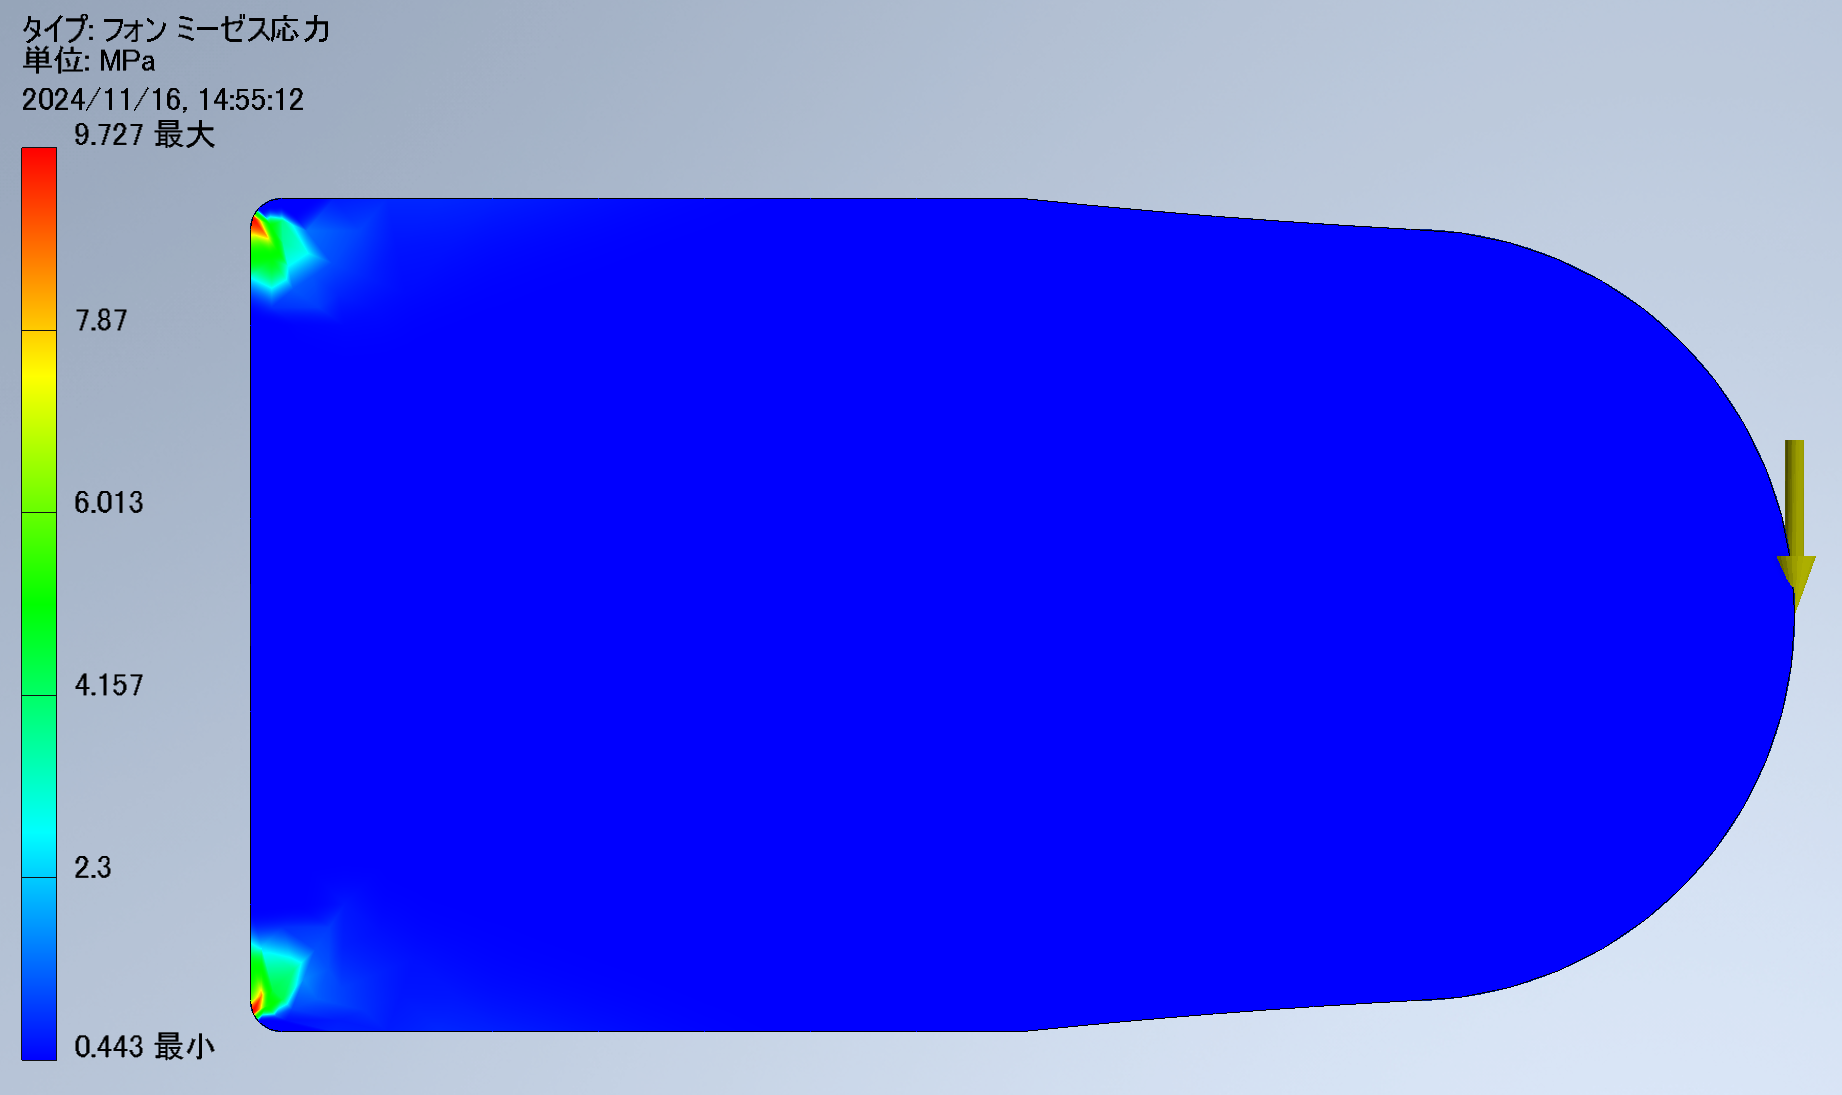
\includegraphics[width=0.99\linewidth]{images/5_voms.png}
        \caption{応力}
        \label{img:5_voms}
      \end{minipage}
      \begin{minipage}{.5\textwidth}
        \centering
        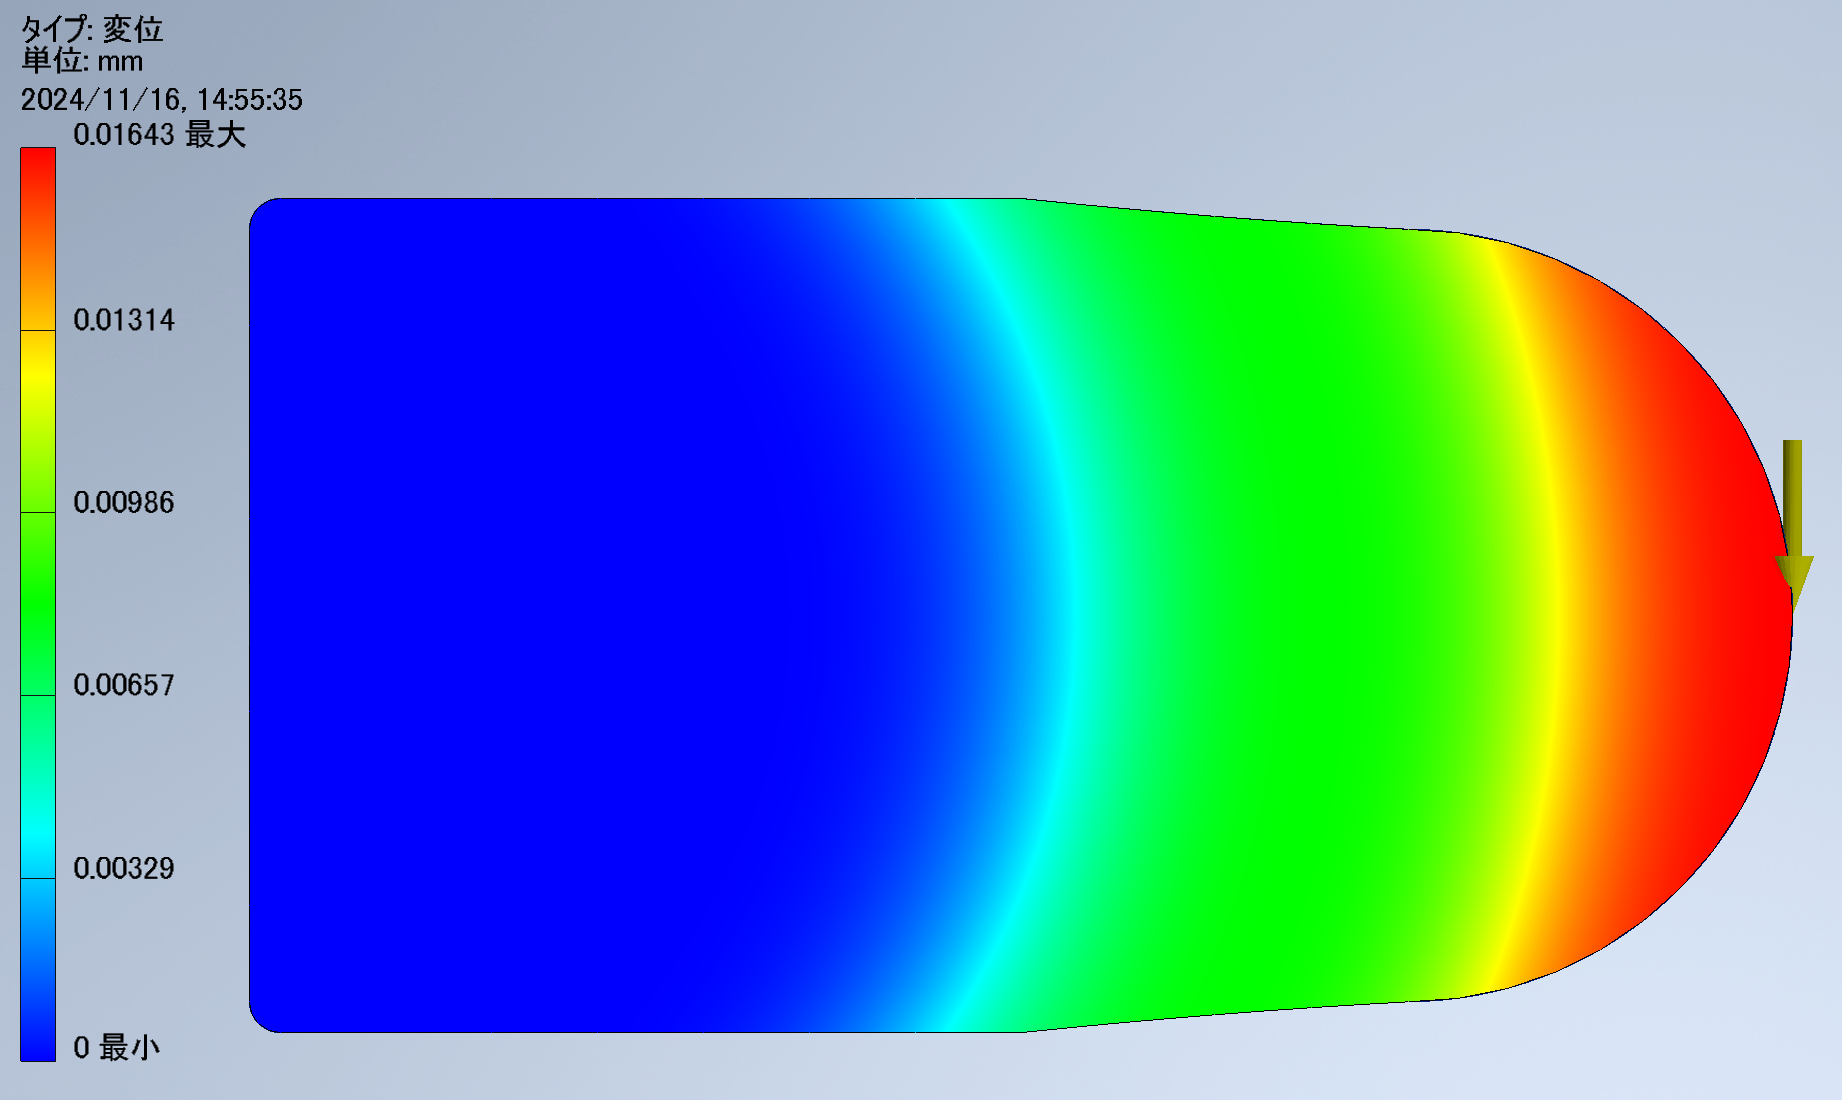
\includegraphics[width=0.99\linewidth]{images/5_disp.png}
        \caption{変位}
        \label{img:5_disp}
      \end{minipage}
    \end{tabular}
  \end{figure}

  以上の図は$100 \times 4[mm^3]$のパーツで補強した梁を,
  更に,応力が一番かかっていた補強パーツと梁の角にフィレットを施して,実験をした結果である.
  解析条件は以下.
  \begin{equation*}
    V \approx 49517[mm^3]
  \end{equation*}

  図\ref{img:5_disp}より変位の最小値が$0.001643[mm]$になった.
  以下安全率.
  \begin{figure}[H]
    \centering
    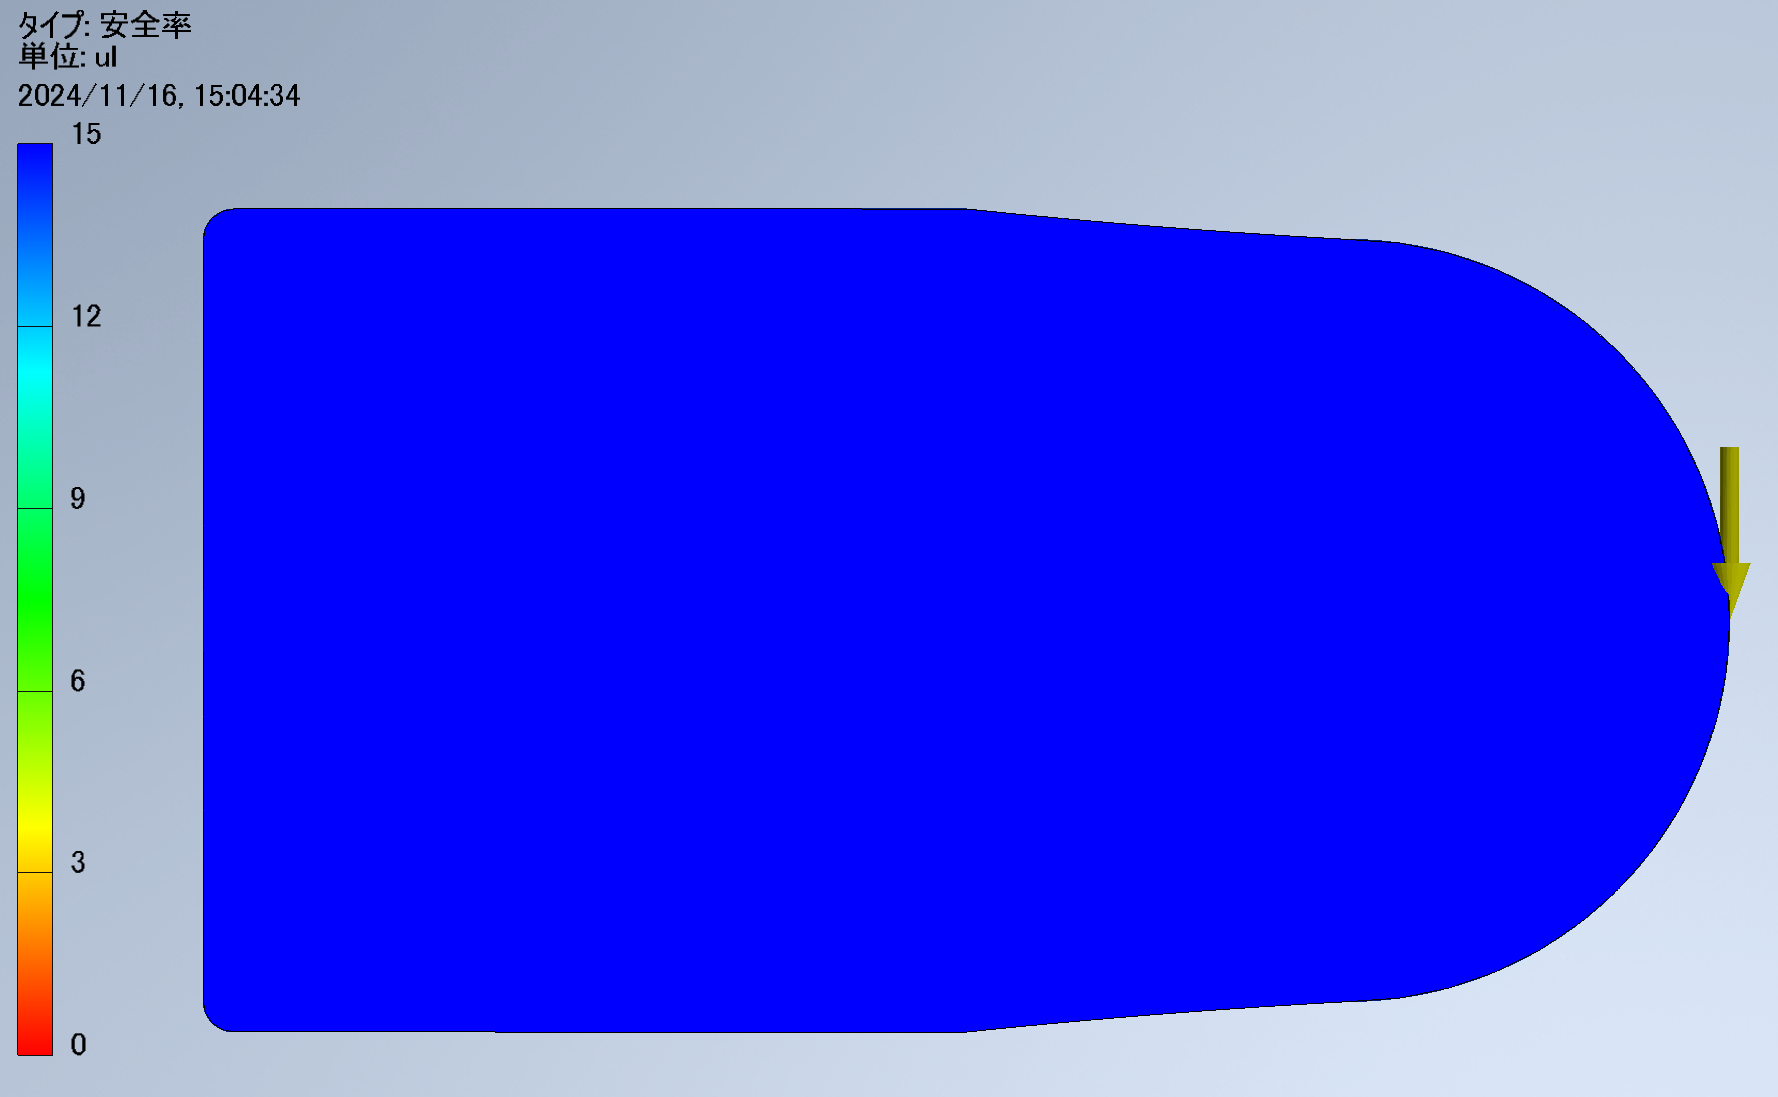
\includegraphics[width=0.5\linewidth]{images/5_safe.png}
    \caption{安全率}
    \label{img:5_safe}
  \end{figure}

  最後に課題2の実験を行う.
  \begin{figure}[H]
    \begin{tabular}{ccc}
      \begin{minipage}{.33\textwidth}
        \centering
        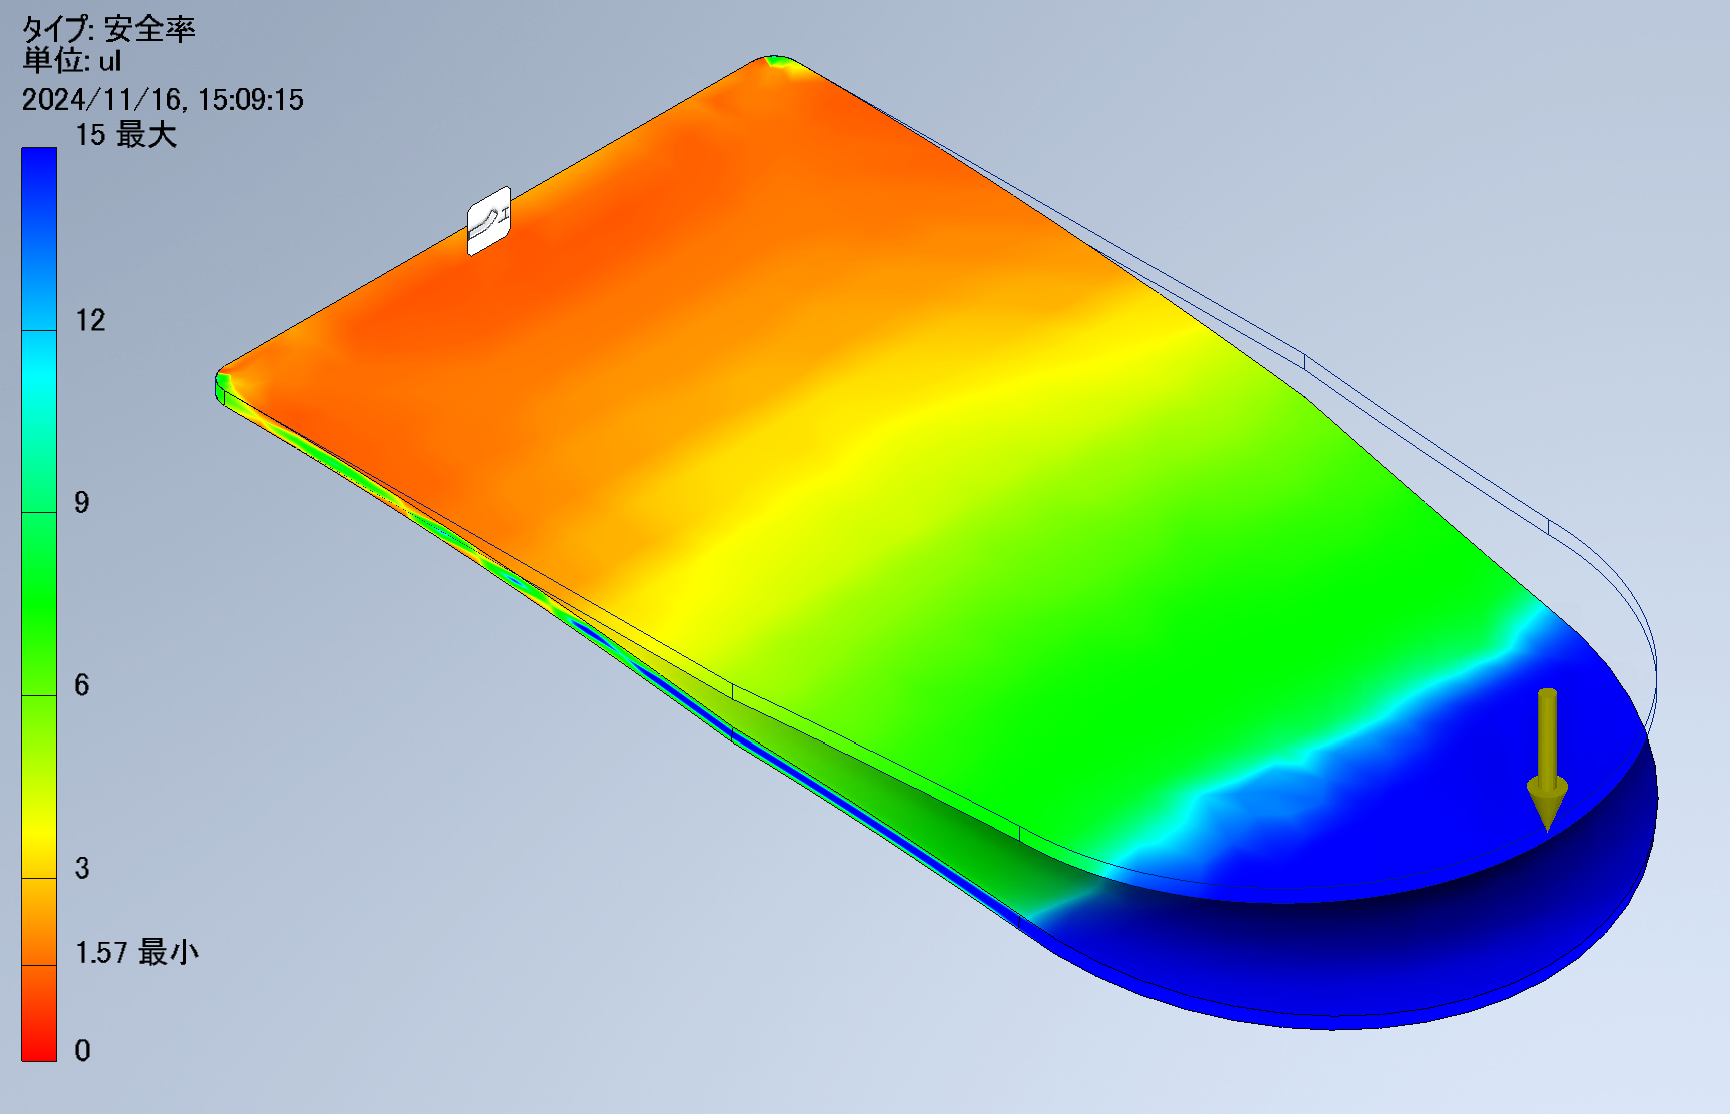
\includegraphics[width=0.99\linewidth]{images/5-1_safe.png}
        \caption{安全率}
        \label{img:5-1_safe}
      \end{minipage}
      \begin{minipage}{.33\textwidth}
        \centering
        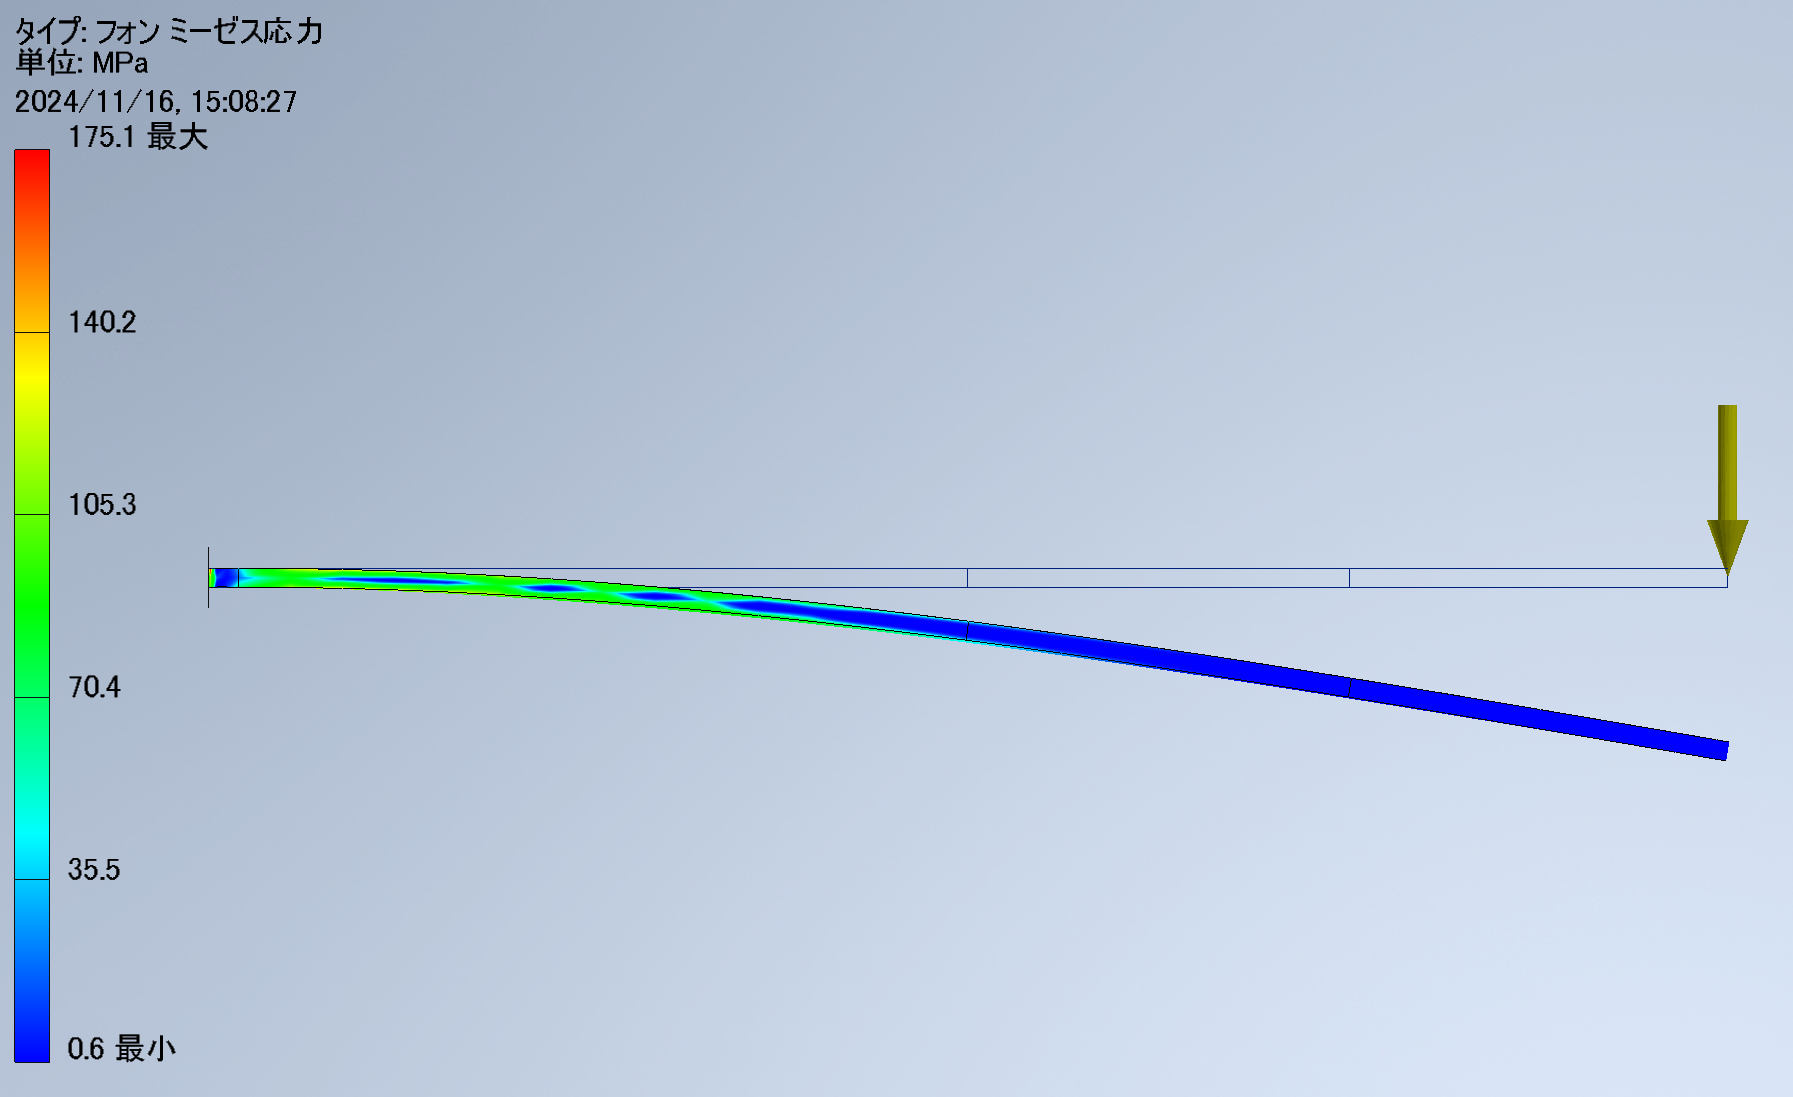
\includegraphics[width=0.99\linewidth]{images/5-1_voms.png}
        \caption{応力}
        \label{img:5-1_voms}
      \end{minipage}
      \begin{minipage}{.33\textwidth}
        \centering
        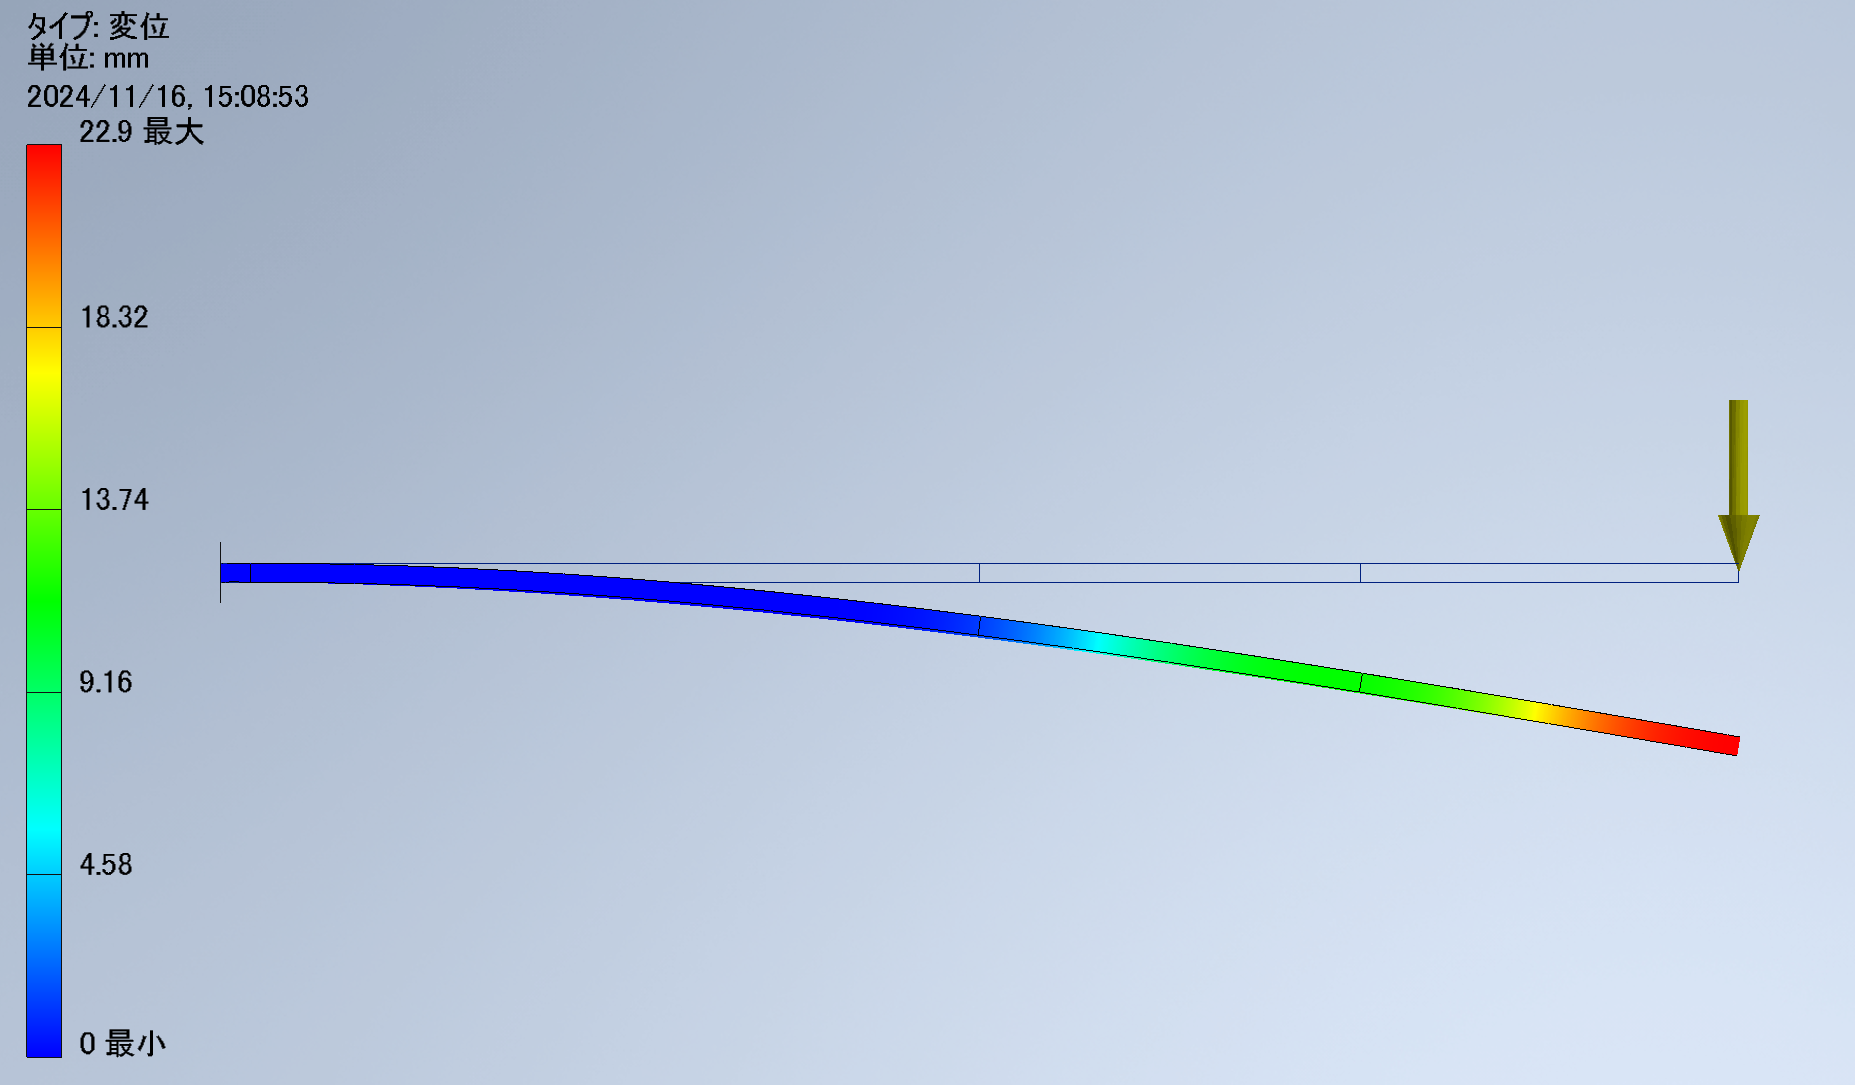
\includegraphics[width=0.99\linewidth]{images/5-1_disp.png}
        \caption{変位}
        \label{img:5-1_disp}
      \end{minipage}
    \end{tabular}
  \end{figure}
